%--------------------------------------------------------------------------------
%
%
%--------------------------------------------------------------------------------
\chapter*{Processing Resources}
\addcontentsline{toc}{chapter}{Processing Resources}




\section*{Data Types}
\addcontentsline{toc}{section}{Data Types}

Twin-64 is a big endian 64-bit machine. The fundamental data type is a 64-bit signed integer with the most significant bit being left. Bits are numbered from left to right, starting with bit 64 as the MSB bit down to bit 0 as LSB. Memory access is performed on a double, word, half-word or byte basis. All addresses are however always expressed as bytes addresses.

\begin{figure}[ht]
\begin{center}
\begin{tikzpicture}[scale=0.7, transform shape]
        
  	\draw[help lines, gray!70, dashed] (0,0) grid(16,8);
  	
  	\node[  tsRectangle, 
            minimum width=4cm,
            minimum height=0.75cm,
            fill=white!50] (blocks) at (14,7) { Byte };
                
    \node at (15.75,7.75) {0};
    \node at (12.25,7.75) {7};

    \node[  tsRectangle, 
            minimum width=8cm,
            minimum height=0.75cm,
            fill=white!50] (blocks) at (12,5) { Half };
                
    \node at (15.75,5.75) {0};
    \node at (8.25,5.75) {15};
       
    \node[  tsRectangle, 
            minimum width=12cm,
            minimum height=0.75cm,
            fill=white!50] (blocks) at (10,3) { Word };
                
    \node at (15.75,3.75) {0};
    \node at (4.25,3.75) {31};
    
    \node[  tsRectangle, 
            minimum width=16cm,
            minimum height=0.75cm,
            fill=white!50] (blocks) at (8,1) { Double };
            
    \node at (15.75,1.75) {0};
    \node at (.25,1.75) {63};
                
      
\end{tikzpicture}
\end{center}
\caption{Data types}
\label{fig:data types}
\end{figure}


lower sizes are sign extended before use

address computation uses a 32-bit unsigned math, i.e. numbers wrap around in 32 bit space.


\section*{Byte Ordering}
\addcontentsline{toc}{section}{Byte Ordering}

Twin-64 supports little endian and big endian byte ordering models.



\section*{General Registers}
\addcontentsline{toc}{section}{General Registers}

Twin-64 features a set of 16 general purposes registers.

\begin{figure}[H]
\begin{center}
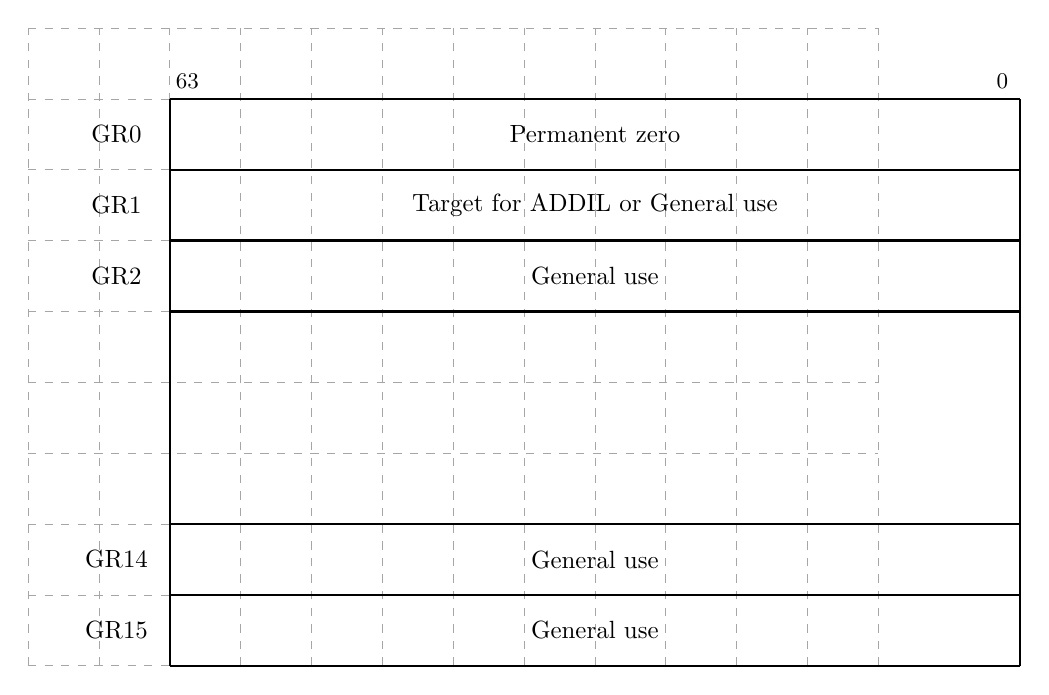
\begin{tikzpicture}[scale=0.9, transform shape]
        
  	\draw[help lines, gray!70, dashed] (0,0) grid(12,9);

	% Rectangle dimensions
	\def\width{12}
	\def\leftofs{2}
	\def\rightofs{\leftofs + \width}
	
	% Bits
	\node at (\leftofs + 0.25,8 + 0.25) {\small 63};
	\node at (\rightofs - 0.25,8 + 0.25) {\small 0};

	% Box
	\draw[thick] (\leftofs, 0) -- (\leftofs, 8);
	\draw[thick] (\rightofs, 0) -- (\rightofs, 8);
	\draw[thick] (\leftofs, 0) -- (\rightofs, 0);
	\draw[thick] (\leftofs, 8) -- (\rightofs, 8);
	  		
	% Fields  		
  	\draw[thick] (\leftofs, 7) -- (\rightofs, 7);
  	\node at ({\leftofs - 0.75}, {7 + 0.5}) { GR0 };
  	\node at (8, {7 + 0.5}) { Permanent zero };
  		
  	\draw[thick] (\leftofs, 6) -- (\rightofs, 6);
  	\node at ({\leftofs - 0.75}, {6 + 0.5}) { GR1};
  	\node at (8, {6 + 0.5}) { Target for ADDIL or General use };	
  		
  	\draw[thick] (\leftofs, 5) -- (\rightofs, 5);
  	\node at ({\leftofs - 0.75}, {5 + 0.5}) { GR2};
  	\node at (8, {5 + 0.5}) { General use };	
  		
  	\draw[thick] (\leftofs, 2) -- (\rightofs, 2);
  	\node at ({\leftofs - 0.75}, {1 + 0.5}) { GR14};
  	\node at (8, {1 + 0.5}) { General use };	
  		
  	\draw[thick] (\leftofs, 1) -- (\rightofs, 1);
  	\node at ({\leftofs - 0.75}, {0 + 0.5}) { GR15};
  	\node at (8, {0 + 0.5}) { General use };	
  
\end{tikzpicture}
\end{center}
\caption{General registers}
\label{fig:General registers}
\end{figure}

Some general registers have a dedicated use. Register zero will always return a zero value when read and a write operation will have no effect. Although there are only 16 general registers in the CPU, implementing such a register greatly simplifies the instruction design, in that it for example provides a target when the result is not needed. General register one is a scratch register and also serves as an implicit target for some instructions. Other general registers may have dedicated purpose defined in the runtime architecture. 

\section*{Control Registers}
\addcontentsline{toc}{section}{Control Registers}

\begin{figure}[H]
\begin{center}
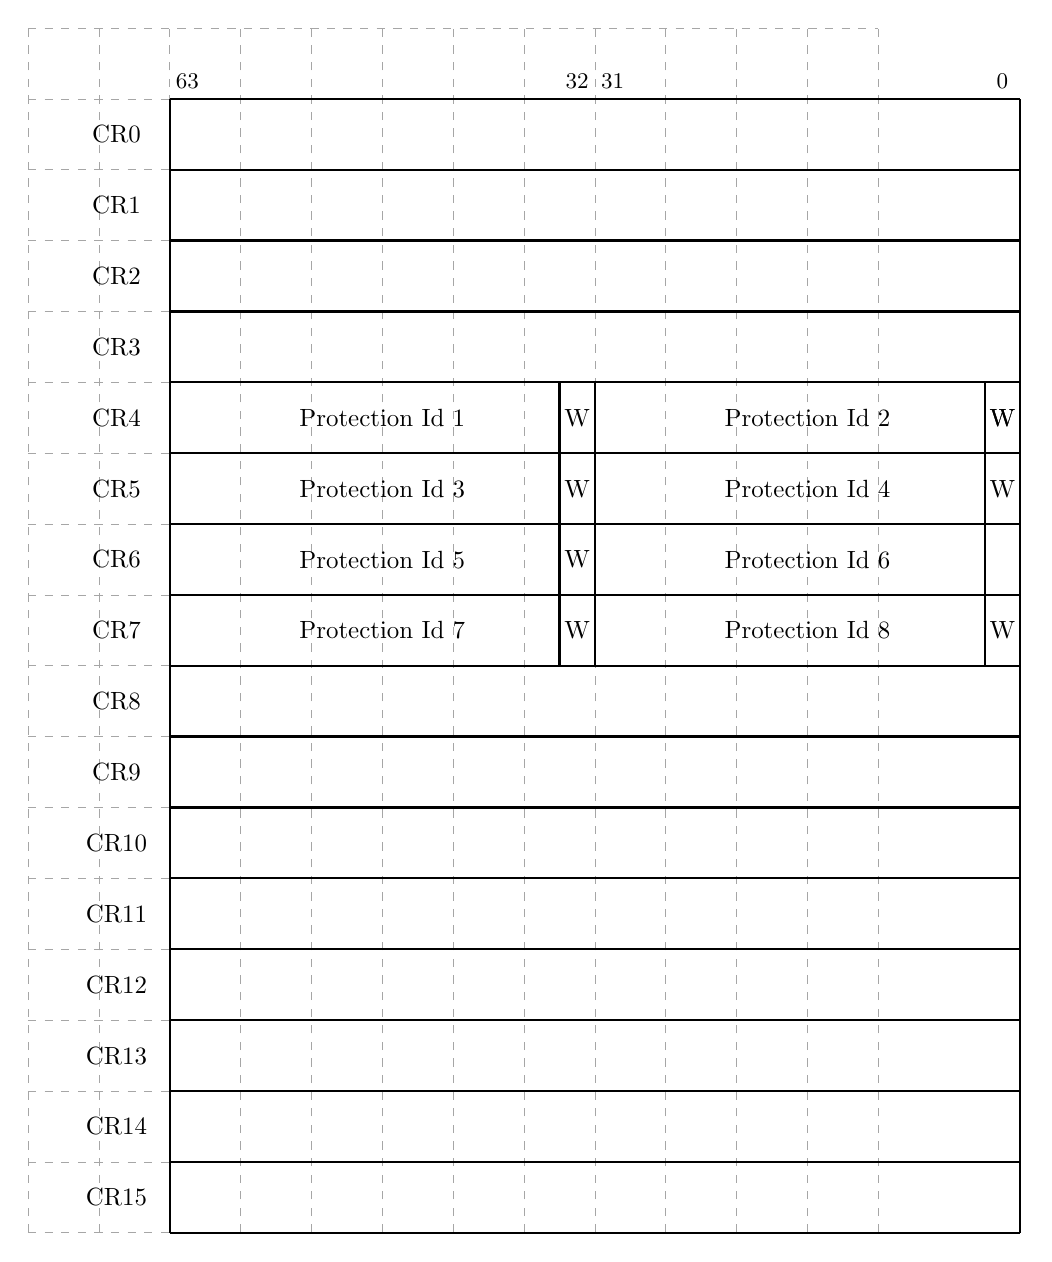
\begin{tikzpicture}[scale=0.9, transform shape]
        
  	\draw[help lines, gray!70, dashed] (0,0) grid(12,17);
  	
  	% Rectangle dimensions
	\def\width{12}
	\def\leftofs{2}
	\def\rightofs{\leftofs + \width}
  	
  	% Bits
  	\node at (\leftofs + 0.25,16 + 0.25) {\small 63};
  	\node at (\leftofs + 5.75,16 + 0.25) {\small 32};
	\node at (\rightofs - 5.75,16 + 0.25) {\small 31};
	\node at (\rightofs - 0.25,16 + 0.25) {\small 0};

	% Box
	\draw[thick] (\leftofs, 0) -- (\leftofs, 16);
	\draw[thick] (\rightofs, 0) -- (\rightofs, 16);
	\draw[thick] (\leftofs, 0) -- (\rightofs, 0);
	\draw[thick] (\leftofs, 16) -- (\rightofs, 16);
	
	% Fields 
	% CR0
	\draw[thick] (\leftofs, 15) -- (\rightofs, 15);
  	\node at ({\leftofs - 0.75}, {15 + 0.5}) { CR0 };
  	
  	% CR1
  	\draw[thick] (\leftofs, 14) -- (\rightofs, 14);
  	\node at ({\leftofs - 0.75}, {14 + 0.5}) { CR1 };
  	
  	% CR2
  	\draw[thick] (\leftofs, 13) -- (\rightofs, 13);
  	\node at ({\leftofs - 0.75}, {13 + 0.5}) { CR2 };
  	
  	% CR3
  	\draw[thick] (\leftofs, 12) -- (\rightofs, 12);
  	\node at ({\leftofs - 0.75}, {12 + 0.5}) { CR3 };
  	
  	% CR4
  	\draw[thick] (\leftofs, 11) -- (\rightofs, 11);
  	\draw[thick] (\leftofs + \width / 2, 11) -- (\leftofs + \width / 2, 12);
  	\draw[thick] (\leftofs + \width / 2 - 0.5, 11) -- (\leftofs + \width / 2 - 0.5, 12);
  	\draw[thick] (\rightofs - 0.5, 11) -- (\rightofs - 0.5, 12);
  	\node at ({\leftofs - 0.75}, {11 + 0.5}) { CR4 };
  	\node at ({\leftofs + 3}, {11 + 0.5}) { Protection Id 1 };
  	\node at ({\leftofs + \width/2 - 0.25}, {11 + 0.5}) { W };
  	\node at ({\rightofs - 3}, {11 + 0.5}) { Protection Id 2 };
  	\node at ({\rightofs - 0.25}, {11 + 0.5}) { W };
  	
  	% CR5
  	\draw[thick] (\leftofs, 10) -- (\rightofs, 10);
  	\draw[thick] (\leftofs + \width / 2, 10) -- (\leftofs + \width / 2, 11);
  	\draw[thick] (\leftofs + \width / 2 - 0.5, 10) -- (\leftofs + \width / 2 - 0.5, 11);
  	\draw[thick] (\rightofs - 0.5, 10) -- (\rightofs - 0.5, 11);
  	\node at ({\leftofs - 0.75}, {10 + 0.5}) { CR5 };
  	\node at ({\leftofs + 3}, {10 + 0.5}) { Protection Id 3 };
  	\node at ({\leftofs + \width/2 - 0.25}, {10 + 0.5}) { W };
  	\node at ({\rightofs - 3}, {10 + 0.5}) { Protection Id 4 };
  	\node at ({\rightofs - 0.25}, {10 + 0.5}) { W };
  	
  	%CR6
  	\draw[thick] (\leftofs, 9) -- (\rightofs, 9);
  	\draw[thick] (\leftofs + \width / 2, 9) -- (\leftofs + \width / 2, 10);
  	\draw[thick] (\leftofs + \width / 2 - 0.5, 9) -- (\leftofs + \width / 2 - 0.5, 10);
  	\draw[thick] (\rightofs - 0.5, 9) -- (\rightofs - 0.5, 10);
  	\node at ({\leftofs - 0.75}, {9 + 0.5}) { CR6 };
  	\node at ({\leftofs + 3}, {9 + 0.5}) { Protection Id 5 };
  	\node at ({\leftofs + \width/2 - 0.25}, {9 + 0.5}) { W };
  	\node at ({\rightofs - 3}, {9 + 0.5}) { Protection Id 6 };
  	\node at ({\rightofs - 0.25}, {11 + 0.5}) { W };
  	
  	% CR7
  	\draw[thick] (\leftofs, 8) -- (\rightofs, 8);
  	\draw[thick] (\leftofs + \width / 2, 8) -- (\leftofs + \width / 2, 9);
  	\draw[thick] (\leftofs + \width / 2 - 0.5, 8) -- (\leftofs + \width / 2 - 0.5, 9);
  	\draw[thick] (\rightofs - 0.5, 8) -- (\rightofs - 0.5, 9);
  	\node at ({\leftofs - 0.75}, {8 + 0.5}) { CR7 };
  	\node at ({\leftofs + 3}, {8 + 0.5}) { Protection Id 7 };
  	\node at ({\leftofs + \width/2 - 0.25}, {8 + 0.5}) { W };
  	\node at ({\rightofs - 3}, {8 + 0.5}) { Protection Id 8 };
  	\node at ({\rightofs - 0.25}, {8 + 0.5}) { W };
  	
  	% CR8
  	\draw[thick] (\leftofs, 7) -- (\rightofs, 7);
  	\node at ({\leftofs - 0.75}, {7 + 0.5}) { CR8 };
  	
  	% CR9
  	\draw[thick] (\leftofs, 6) -- (\rightofs, 6);
  	\node at ({\leftofs - 0.75}, {6 + 0.5}) { CR9 };
  	
  	% CR10
  	\draw[thick] (\leftofs, 5) -- (\rightofs, 5);
  	\node at ({\leftofs - 0.75}, {5 + 0.5}) { CR10 };
  	
  	% CR11
  	\draw[thick] (\leftofs, 4) -- (\rightofs, 4);
  	\node at ({\leftofs - 0.75}, {4 + 0.5}) { CR11 };
  	
  	% CR12
  	\draw[thick] (\leftofs, 3) -- (\rightofs, 3);
  	\node at ({\leftofs - 0.75}, {3 + 0.5}) { CR12 };
  	
  	% CR13
  	\draw[thick] (\leftofs, 2) -- (\rightofs, 2);
  	\node at ({\leftofs - 0.75}, {2 + 0.5}) { CR13 };
  	
  	% CR14
  	\draw[thick] (\leftofs, 1) -- (\rightofs, 1);;
  	\node at ({\leftofs - 0.75}, {1 + 0.5}) { CR14 };
  	
  	% CR15
  	\draw[thick] (\leftofs, 0) -- (\rightofs, 0);
  	\node at ({\leftofs - 0.75}, {0 + 0.5}) { CR15 };
			
\end{tikzpicture}
\end{center}
\caption{Control registers}
\label{fig:Control registers}
\end{figure}



\section*{Program State Register}
\addcontentsline{toc}{section}{Processor State Register}


\begin{figure}[H]
\begin{center}
\begin{tikzpicture}[scale=0.9, transform shape]
        
  	\draw[help lines, gray!70, dashed] (0,0) grid(16,1.5);
  	
    \node[  tsRectangle, 
            minimum width=16cm,
            minimum height=1cm,  
            fill=white!50] (blocks) at (8,1) { };
                
  	\draw[-] (0.25,0.5) -- (0.25,1.5);
    \draw[-] (0.5,0.5) -- (0.5,1.5);
    \draw[-] (0.75,0.5) -- (0.75,1.5);
    \draw[-] (1,0.5) -- (1,1.5);
  	\draw[-] (1.25,0.5) -- (1.25,1.5);
    \draw[-] (1.5,0.5) -- (1.5,1.5);
   	\draw[-] (1.75,0.5) -- (1.75,1.5);
   	\draw[-] (2,0.5) -- (2,1.5);
   	\draw[-] (2.25,0.5) -- (2.25,1.5);
   	\draw[-] (2.5,0.5) -- (2.5,1.5);
   	\draw[-] (2.75,0.5) -- (2.75,1.5);	     	
   	\draw[-] (3,0.5) -- (3,1.5);
    \draw[-] (8,0.5) -- (8,1.5);
     	
    \def\flagOfs{0.125}
	\node at (\flagOfs, 1) {\tiny X};
	\node at (\flagOfs + 0.25, 1) {\tiny X};
	\node at (\flagOfs + 0.5, 1) {\tiny X};
	\node at (\flagOfs + 0.75, 1) {\tiny X};
	\node at (\flagOfs + 1, 1) {\tiny X};
	\node at (\flagOfs + 1.25, 1) {\tiny X};
	\node at (\flagOfs + 1.5, 1) {\tiny X};
	\node at (\flagOfs + 1.75, 1) {\tiny X};
	\node at (\flagOfs + 2, 1) {\tiny X};
	\node at (\flagOfs + 2.25, 1) {\tiny X};
	\node at (\flagOfs + 2.5, 1) {\tiny X};
	\node at (\flagOfs + 2.75, 1) {\tiny X};
				
	\node at (5.75,1) {\small IA Segment};
	\node at (11,1) {\small IA Offset};
		
	\node at (1.5,0.25) {12};
    \node at (5,0.25) {20};
   	\node at (11,0.25) {32};
   	 	
\end{tikzpicture}
\end{center}
\caption{Program state register}
\label{fig:Program state register}
\end{figure}

\begin{longtable}{@{}p{0.25\linewidth}p{0.6\linewidth}@{}}
    \caption{Status Field Bits} \\
    \toprule
    \textbf{Head 1} & \textbf{Head 2} \\
    \midrule
    \endfirsthead
    \toprule
    \textbf{Head 1} & \textbf{Head 2} \\
    \midrule
    \endhead
    \midrule
    \multicolumn{2}{r}{\textit{Continued on next page}} \\
    \midrule
    \endfoot
    \bottomrule
    \endlastfoot
    \textbf{text 1} & text \\
    \midrule
    \textbf{text 2} & text \\
\end{longtable}



\section*{TLB}
\addcontentsline{toc}{section}{TLB}

For performance reasons, the virtual address translation result is stored in a translation look-aside buffer. The TLB is essentially a copy of the page table entry information that represents the virtual page currently loaded at the physical address. Depending on the hardware implementation, there can be a combined TLB or a separate instruction TLB and data TLB. A TLB is essentially a cache for address translations. The virtual page number, VPN, is stored along with attributes and the physical page number, PPN, in the TLB hardware. The current architecture allows for a 34-bit physical address space, which is a 16GB memory space.

\begin{figure}[H]
\begin{center}
\begin{tikzpicture}[scale=0.9, transform shape]
        
  	\draw[help lines, gray!70, dashed] (0,0) grid(16,6);
  	
    \node[  tsRectangle, 
            minimum width=9.5cm,
            minimum height=0.75cm,  
            fill=white,
            anchor=west] at (0,5) { };
    \node[anchor=west] at (0, 5) {\small Virtual page number};
    \node[anchor=west] at (11,5) {38bit};
            
  	\node[  tsRectangle, 
            minimum width=5cm,
            minimum height=0.75cm,  
            fill=white,
            anchor=west] at (0,4) { };
    \node[anchor=west] at (0, 4) {\small Physical page number};   
     \node[anchor=west] at (11,4) {20bit};
    
    \node[  tsRectangle, 
            minimum width=8cm,
            minimum height=0.75cm,  
            fill=white,
            anchor=west] at (0,3) { };
    \draw[-] (7.75,2.625) -- (7.75,3.35);
    \node[anchor=west] at (0, 3) {\small Protection ID};  
    \node[anchor=west] at (7.65, 3) {\tiny W};  
    \node[anchor=west] at (11,3) {32bit};
     
    \node[  tsRectangle, 
            minimum width=1cm,
            minimum height=0.75cm,  
            fill=white,
            anchor=west] at (0,2) { };
    \node[anchor=west] at (0, 2) {\small Acc}; 
    \node[anchor=west] at (11,2) {4bit};
    
    \node[  tsRectangle, 
            minimum width=2cm,
            minimum height=0.75cm,  
            fill=white,
            anchor=west] at (0,1) { };
    \node[anchor=west] at (0,1) {\small Flags};
    \node[anchor=west] at (11,1) {8bit};
            
\end{tikzpicture}
\end{center}
\caption{Tlb info}
\label{fig: Tlb info}
\end{figure}


The first four segments, segment 0 to 3, are special in that they bypass the TLB entirely. The address range represents physical memory and can only be access in privileged mode. A virtual address in the range 0x00\_0000\_0000 to 0x03\_FFFF\_FFFF directly maps to the physical address of the same range.

To reduce TLB processing overhead, the TLB is capable of storing virtual address ranges. There is support for a large page size of 16Kb, 256 Kb, 4Mb and 64 Mb.



38bit VPN, 20bit PPN, 4bit AR, 32 bit PID, 2bit size, xbit flags


bits:

V - valid

L - entry locked

M - modified trap

B - branch taken trap

U - uncacheable

\begin{longtable}{@{}p{0.25\linewidth}p{0.6\linewidth}@{}}
    \caption{TLB Fields} \\
    \toprule
    \textbf{Head 1} & \textbf{Head 2} \\
    \midrule
    \endfirsthead
    \toprule
    \textbf{Head 1} & \textbf{Head 2} \\
    \midrule
    \endhead
    \midrule
    \multicolumn{2}{r}{\textit{Continued on next page}} \\
    \midrule
    \endfoot
    \bottomrule
    \endlastfoot
    \textbf{text 1} & text \\
    \midrule
    \textbf{text 2} & text \\
\end{longtable}






\section*{Caches}
\addcontentsline{toc}{section}{Caches}

Twin-64 is a cache visible architecture, featuring cache models for unified or separate instruction and data cache. While hardware directly controls the cache for cache line insertion and replacement, the software has explicit control on flushing and purging cache line entries. There are instructions to flush and purge cache lines. To speed up the entire memory access process, the cache uses the virtual address to index into the arrays, which can be done in parallel to the TLB lookup. When the physical address tag in the cache and the physical page address in the TLB match, there will be a cache hit. The architecture will not specify the size of cache lines or cache organization. Typically a cache line will hold four to eight machine words, the cache organization is in the simplest case a single set direct mapped cache. The Twin-64 architecture does not specify a particular cache and cache hierarchy model. The architecture just specifies instructions to handle cache operations, such as delete or flushing a cache.

